  %%%%%%%%%%%%%%%%%%%%%%%%%%%%%%%%%%%%%%%%%%%%%%%%%%%%%%%%%%%%%%%%%%%%%%
% LaTeX Example: Project Report

%%% Preamble
\documentclass[paper=a4, fontsize=12pt, abstract=on]{scrartcl}
\usepackage[T1]{fontenc}
\usepackage{fourier}
\usepackage{tabularx}
\usepackage[utf8]{inputenc}
\usepackage{hyperref}





\usepackage{listings}
\usepackage{color}

\definecolor{dkgreen}{rgb}{0,0.6,0}
\definecolor{gray}{rgb}{0.5,0.5,0.5}
\definecolor{mauve}{rgb}{0.58,0,0.82}
\lstset{frame=tb,
  language=[Visual]C++,
  aboveskip=3mm,
  belowskip=3mm,
  showstringspaces=false,
  columns=flexible,
  basicstyle={\small\ttfamily},
  numbers=none,
  numberstyle=\tiny\color{gray},
  keywordstyle=\color{blue},
  commentstyle=\color{dkgreen},
  stringstyle=\color{mauve},
  breaklines=true,
  breakatwhitespace=true,
  tabsize=3
}
\usepackage{graphicx}
\usepackage{caption}
\usepackage{subcaption}

\usepackage[english]{babel}															% English language/hyphenation
\usepackage[protrusion=true,expansion=true]{microtype}	
\usepackage{amsmath,amsfonts,amsthm} % Math packages

\usepackage{url}
%\usepackage[hang, small,labelfont=bf,up,textfont=it,up]{caption}


%%% Custom sectioning
\usepackage{sectsty}
\allsectionsfont{\normalfont\scshape}
\usepackage{float}
\usepackage{amsmath}
\usepackage{mathtools}
\usepackage{ragged2e}

\usepackage{nomencl}
\makenomenclature

%%% Custom headers/footers (fancyhdr package)
\usepackage{fancyhdr}
\pagestyle{fancyplain}
\fancyhead{}											% No page header
\fancyfoot[L]{}											% Empty 
\fancyfoot[C]{}											% Empty
\fancyfoot[R]{\thepage}									% Pagenumbering
\renewcommand{\headrulewidth}{0pt}			% Remove header underlines
\renewcommand{\footrulewidth}{0pt}				% Remove footer underlines
\setlength{\headheight}{13.6pt}
   \renewcommand*\abstractname{Summary}

%%% Equation and float numbering
\numberwithin{equation}{section}		% Equationnumbering: section.eq#
\numberwithin{figure}{section}			% Figurenumbering: section.fig#
\numberwithin{table}{section}				% Tablenumbering: section.tab#


%%% Maketitle metadata

\newcommand{\horrule}[1]{\rule{\linewidth}{#1}} 	% Horizontal rule

\title{
		%\vspace{-1in} 	
		\usefont{OT1}{bch}{b}{n}
		\normalfont \normalsize \textsc{} \\ [25pt]
		
\includegraphics[width=0.3\linewidth]{ubc.png} \\
		%
\includegraphics[width=0.4\linewidth]{tru}		
		\horrule{0.5pt} \\[0.2cm]
		\huge 502 Mini-Project \#2 : Flow due to Oscillating Plate  \\
		\horrule{2pt} \\[0.005cm]
}
\author{
		\normalfont 								\normalsize
        Jerin Roberts\\[-5pt]		\normalsize
        \today
}
\date{}




%%% Begin document
\begin{document}
\maketitle
\begin{center}
\begin{tabular}{l r}


Supervisor: & Dr. Dana Grecov  \\ % supervisor
Locations: & University of British Columbia


\end{tabular}
\end{center}



\newpage
\tableofcontents
\listoffigures
\listoftables
\newpage
\lstset{language=[Visual]C++}
\section{Overview}



 The problem of an oscillating plate flows has lots of applications in a variety of engineering and biological fields and hence such flows have been investigated researchers. Stokes has discussed the motion of a fluid in contact with a harmonically vibrating plate and has since been known as stokes 2nd problem. Since then many authors have studied the flow of a fluid on oscillating flat plates and through oscillating channels of various geometries.  In this paper the flow of an incompressible viscous fluid on an infinite harmonically oscillating plate is considered The technique adopted is of that used in the classical Stokes' second problem.
\section{Problem}
First lets consider an infinite flat plate containing an infinite dept of fluid relative to the affect range. The plate executes sinusoidal oscillations parallel to the itself as shown in the diagram \ref{osc}.

\begin{figure}[H]
\centering
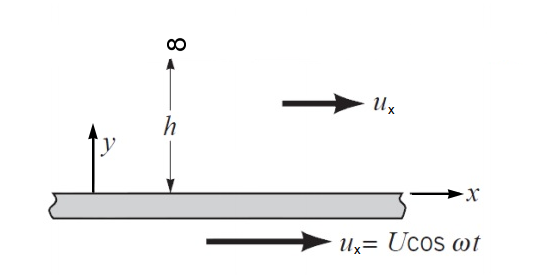
\includegraphics[width=0.85\linewidth]{di}
\caption{Diagram of infinite plate and fluid for problem}
\label{osc}
\end{figure}



 The problem is to find a solution to the flow after all transients have died out. This simplifies the problem as there are no initial conditions to satisfy. This problem is often referred to as stokes second problem. We begin solving by finding the simplified governing equations from the generalized 2D differential navier stokes equations \ref{nav}. 

 \begin{equation}
\label{gov}
\frac{\partial u}{\partial x}+\frac{\partial v}{\partial y} = 0
\end{equation} 

 \begin{equation}
\label{nav}
\frac{\partial u}{\partial t} +u\frac{\partial u}{\partial x}+v\frac{\partial u}{\partial y} = -\frac{1}{\rho}\frac{\partial P}{\partial x} + g_x + \eta \Bigg(  \frac{\partial^2 u}{\partial x^2} + \frac{\partial^2 u}{\partial y^2} \Bigg)
\end{equation} 

 \begin{equation}
\label{gov}
\frac{\partial v}{\partial t} +u\frac{\partial v}{\partial x}+v\frac{\partial v}{\partial y} = -\frac{1}{\rho}\frac{\partial P}{\partial x} + g_y + \eta \Bigg( \frac{\partial^2 v}{\partial y^2} +  \frac{\partial^2 v}{\partial y^2} \Bigg)
\end{equation} 

This can written as a 1D problem as we are only concerned with the velocity profile $u_x$ in the y direction, ie $u_z$ and $u_y$ are considered to be small and equal to zero. We don't expect a pressure gradient in the x direction because of the infinite dimension of the plate. A pressure gradient in the y direction will be due only to gravity which we are ignoring for this problem. These assumptions lead to many cancellations and result in the governing equations \ref{gov} used to solve the problem


 \begin{equation}
\label{gov}
\frac{\partial u}{\partial t} = \eta \frac{\partial^2 u}{\partial y^2}
\end{equation} 


The boundary conditions exist at the plate and far away from the plate. Near the plate we require a no slip condition, therefore the velocity of the flow at the plate is equal to its sinusoidal motion. The motion is expect to decay as one moves away from the plate were the fluid motion is zero. The boundary conditions are shown below.

 \begin{equation}
\label{b1}
u(0,t) = U\cos \omega t
\end{equation}

 
  \begin{equation}
\label{b2}
u(0,\infty) = 0
\end{equation}

\section{Solving}
Based on the governing equations we expect the solution to take on the form of equation \ref{f} which suggests this can be solved using separation of variables.
\begin{equation}
\label{51}
u = g(t)f(y)
\end{equation}
Since the period of the oscillations of the plate introduces a time scale, no similarity solution exists to this problem. By considering the equations governing the fluid it may be expected that $u_x$ will also oscillate with the same frequency relative to the movement of the plate, with however a phase shift due to the shear slip between fluid layers. In the steady state therefore the flow variables must have a periodicity equivalent to the periodicity of the motion of the plate. Therefore we will consider a separable solution of the form shown in equation \ref{51}.

 \begin{equation}
\label{51}
u = e^{i\omega t}f(y)
\end{equation}


The solution will be considered the real part of the right-hand side. Because $f(y)$ is complex the velocity of the fluid $u(y,t)$ is able to have a phase difference relative to the wall velocity $U\cos \omega t$. To find the solution equation \ref{51} is substituted into the governing equation \ref{gov} which gives

\begin{equation}
\label{52}
i\omega f(y) = \eta \frac{d^2f(y)}{dy^2}
\end{equation}

This is an equation with constant coefficients and must have exponential solutions. Substitution of a solution of the form $f = exp(ky)$ gives $k = \sqrt{i\omega / \eta} \pm(i+1) \sqrt{\omega /2 \eta}$ where the two square roots of $i$ have been used. As a result the solution of equation \ref{53} is


\begin{equation}
\label{53}
f(y) = Ae^{-(1+i)y\sqrt{\omega/2\eta}}+Be^{(1+i)y\sqrt{\omega/2\eta}}
\end{equation}


The condition \ref{b2} requires that the solution for velocity must be zero at $y = \infty$, therefore we find B = 0 in order for this boundary to be satisfied. The solution \ref{51} then becomes

\begin{equation}
\label{54}
u(y,t) = Ae^{i\omega t}e^{-(1+i)y\sqrt{\omega/2\eta}}
\end{equation}


After applying the surface boundary condition \ref{51} due to the oscillating plate we find A to be equal to U. After considering only the real part of equation\ref{54} we finally obtain the velocity distribution over the oscillating plate:

\begin{equation}
\label{55}
u(y,t) = Ue^{-\omega t}\cos\Big(\omega t - y\sqrt{\omega/2\eta}\Big)
\end{equation}

\section{Solution}
The cosine term in equation\ref{55} is generalized as a representation of a wave signal propagating in the direction of y. The exponential term on the other hand represents the amplitude decay in that propagating wave described by the cosine term. The flow therefore resembles a damped wave as displayed in figure \ref{q1}. 


\begin{figure}[H]
\centering
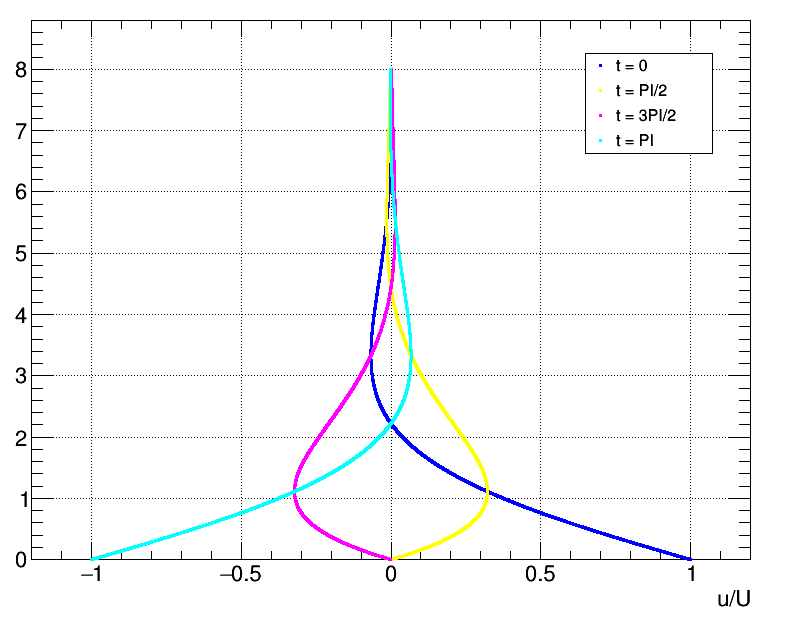
\includegraphics[width=0.70\linewidth]{q1}
\caption{Displays the velocity profile as a function of depth for varying time levels}
\label{q1}
\end{figure}

On an interesting note the problem to be clear is purely a diffusion problem and not wave-propagation problem. This is because there are no restoring forces involved here. The apparent propagation is merely a result of the oscillating boundary condition and the shear coupling between fluid particles. 

\begin{figure}[H]
\centering
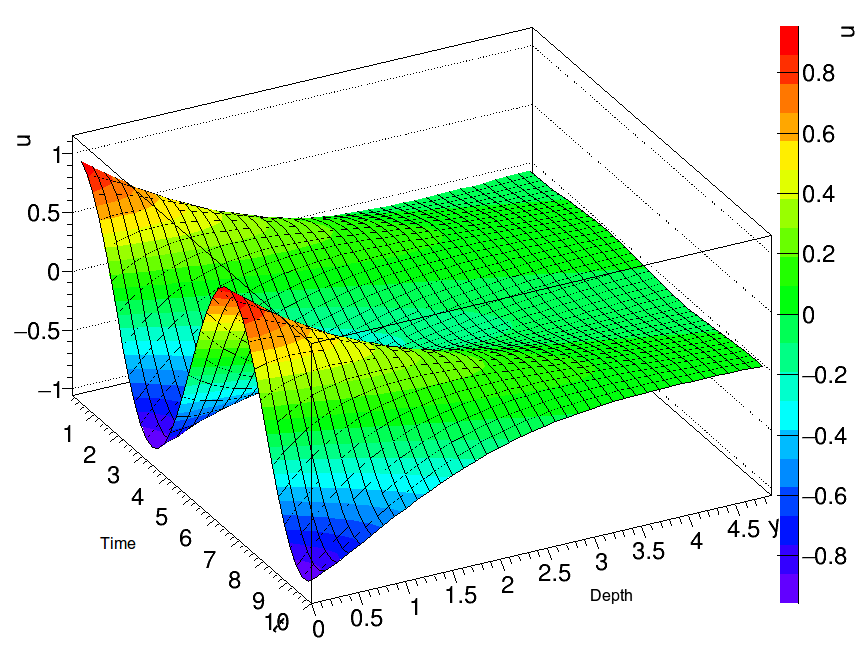
\includegraphics[width=0.70\linewidth]{q2}
\caption{Shows wave propagation as a function of time}
\label{q2}
\end{figure}

The distance at which the wave penetrates into the fluid domain is known as the penetration dept. When we select a value for y far from the wall say, $y = 4\sqrt{\eta/\omega}$, the amplitude of u is $U exp(-4\sqrt{2}) = O.O6U$ which is very small. Therefor we can say the influence of the wall is confined within a distance of approximately:

\begin{equation}
\label{56}
\delta \approx 4\sqrt{\eta/\omega}
\end{equation}

This parameter is known as the depth of penetration dept \cite{g}. This relations suggests that the distance over which the fluid feels the motion of the plate gets smaller as the frequency of the oscillations increases which is displayed in figure \ref{q4}. 


As discussed earlier we noted that the solution \ref{55} cannot be represented by a single curve in terms of the non-dimensional variables. This is expected because the frequency of the boundary motion introduces a natural time scale l/o into the problem, thereby violating the requirements of self-similarity. There are two parameters in the governing set \ref{gov}, namely, U and w. The parameter U can be eliminated by regarding $u / U$ as the dependent variable. 



\begin{figure}[H]
\centering
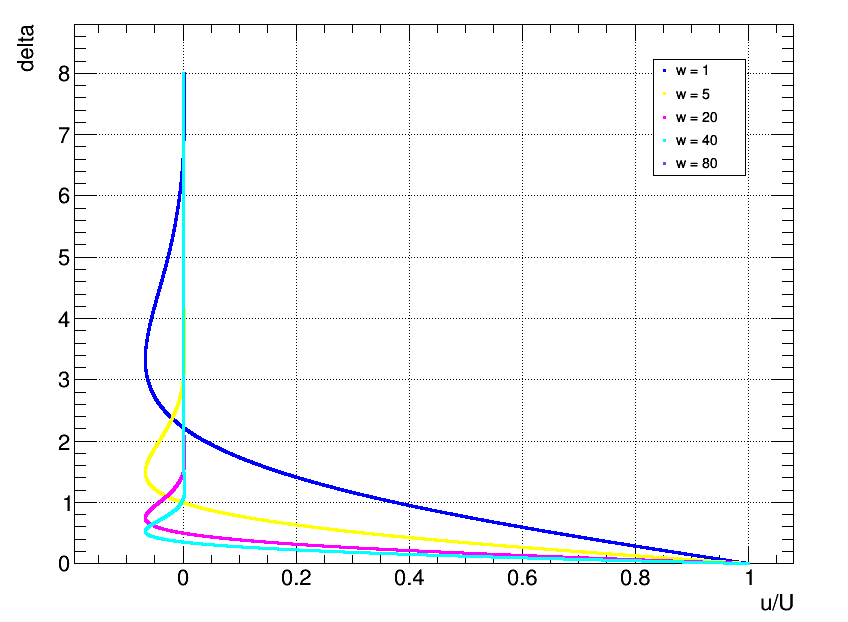
\includegraphics[width=0.70\linewidth]{q4}
\caption{Wave as a function of frequency}
\label{q4}
\end{figure}




It should be noted that the oscillating plate has a constant diffusion distance $\delta = 4\sqrt{\eta/\omega}$ which is only a function of frequency and viscosity. This is very different in contrast to the case of plate started suddenly in which the diffusion distance continues to increases with time. In the problem of sudden acceleration of a plate which shares the same governing equations as that for the oscillating plate,
$\frac{\partial^2 u}{\partial y^2}$ is seen to be positive for all y which results in a positive $\frac{\partial u}{\partial t}$
everywhere. The non varying acceleration indicates that momentum being put into the fluid is not changing direction and therefore is being constantly
diffused outward. This ultimately results in a flow for which its width continues to grow. In the oscillating plate however the $\frac{\partial^2 u}{\partial y^2}$ term varies between positive and negative and therefore $\frac{\partial u}{\partial t}$ constantly changes sign in y and t. Therefore the momentum is unable to diffuse outward like seen in the impulsively started plate which will result in a constant width of flow over time.



\section{Applications}
There are many fields of engineering and science were this flow problem can be applied. 
For fluid problems this solution can be applied in any situation were a periodic linear boundary oscillation occurs. One of such example includes the tank wall of a liquid rocket engine fuel cell. The tank will experience a range of vibrations during flight, and to ensure volatile fuels are not disturbed beyond safety limits the state of the flow near the tank walls can be approximated using this solution. Knowing that the penetration dept is a function of frequency and viscosity engineers will know how much of the fluid is affected near the tank boundary and subsequently which frequencies will require external filtering. 
 In addition to describing flow properties of fluids it can also be used for describing the flow of temperature. In heat conduction the analogous version can be found in that of a semi-infinite solid, the surface of which is subjected to a periodic fluctuation of temperature. The resulting solution (The one explored in this report) has been used to estimate the effective diffuseness in the upper layer of the ocean from measurements of the phase difference between the temperature fluctuations at two
depths which is generated by daily cycle of solar heating from the sun.
One final application and importance of the exact solution is its used for validating numerical methods. When constructing a numerical solution its important to understand its error relative the exact solution. Computation Fluid Dynamic programs specialized for solving complicated fluid problems will have had to validate there system using either analytically or experimental methods. Analytic comparison proves to be the best for determining if the generated software is adequate for solving flow flow problems and provides a benchmark for determining the performance and order of error for the program.



\begin{thebibliography}{99} % Beamer does not support BibTeX so references must be inserted manually as below
\bibitem[Kundu, 2002]{p0}Pijush K. Kundu, Ira M. Cohen
\newblock "Fluid Mechanics, Second Edition",  Department of Mechanical Engineering and Applied Mechanics, University of Pennsylvania, 2002

\bibitem[Sekharan, 1990]{p1}Evelyn Chandra Sekharan; G. Ramanaiah
\newblock "Unsteady Flow Between Two Oscillating Plates",  Faculty of Science, Madras Institute of Technology, Madras-600 044

\bibitem[Papanastasiou, 1999]{p0}Tasos C. Papanastasiou; Georgios C. Georgiou
\newblock "Viscous Fluid Flow",  Department of Mechanical Engineering
Worcester Polytechnic Institute
Worcester, MA

\end{thebibliography}


%%% End document
\end{document}